\section{The term vocabulary} \label{ch3}
We recall that the main steps for constructing an inverted index are:

\begin{enumerate}
    \item Collect the documents;
    \item Tokenize the text;
    \item Do some linguistic pre-processing of the tokens;
    \item Create the inverted index.
\end{enumerate}

In this chapter we first examine the possible formats and aspects of the input document, and then we will focus on the steps of tokenization and linguistic pre-processing of them.

\subsection{Documents}
Digital documents that are the input to an indexing process are typically bytes in a file or on a web server. The first step of processing is then to convert this byte sequence into a linear sequence of characters: however, many formats for the input file exist, along with many different encoding in which the convertion can take place. In this sense, the problem of choosing the best encoding could be addressed by a machine learning algorithm, but it is usually handled heuristically. Moreover, there exist some open source libraries that can handle the presence of multiple languages and formats in a document. Finally, the last issue regards the granularity of the documents: in particular, there's a trade-off between precision of the IR system and the recall. If the units get too small, we are likely to miss important passages because terms were distributed over several mini-documents, while if units are too large we tend to get spurious matches and the relevant information is hard for the user to find. In the following sections we assume that a suitable document size is chosen.

\subsection{Tokenization}
Given a character sequence and a defined document unit, \textbf{tokenization} is the task of chopping it up into pieces, called \textit{tokens}, perhaps at the same time throwing away certain characters, such as punctuation. Despite being often called \textit{terms} or \textit{types}, there's a difference between these entities:

\begin{itemize}
    \item a \textit{token} is an instance of a sequence of characters in some particular document that are grouped together as a useful semantic unit for processing;
    \item a \textit{type} is the class of all tokens containing the same character sequence;
    \item a \textit{term} is a (perhaps normalized) type that is included in the IR system’s dictionary.
\end{itemize}

For example, if the document to be indexed is \textit{to sleep perchance to dream}, then there are 5 tokens, but only 4 types (since there are two instances of \textit{to}). 

Now the question is: what are the correct tokens to use? How do we extract them? In general, for each language there are some tricky cases (e.g. if we have \textit{aren't}, we could tokenize it into \textit{are} and \textit{n't} or \textit{aren} and \textit{t} etc..), and for this reason the \textbf{issues} of tokenization are \textbf{language-specific}. Some examples of issues of tokenization are (more on Chapter 2 of the book):

\begin{itemize}
    \item How to split ambiguous words (e.g. \textit{aren't}, \textit{O'Neill} etc..);
    \item How to deal with special types of characters, such as e-mail addresses, web URLs, IP addresses etc.. A possible solution could be represented by omitting them, resulting on the other hand in restricting a lot what people could search for;
    \item In English, \textit{hyphenation} is a popular technique for splitting up vowels in words or for joining nouns as names; however, handling hyphens automatically could be hard, and it usually done in an heuristic way;
    \item Other language-specific issues (e.g. French, German, Chinese etc..).
\end{itemize}

\subsection{Stop words}
We define \textbf{stop words} as extremely common words (around 30\%) that would appear to be of little value in helping selecting documents matching a user need. The general strategy for determining a \textit{stop list} is to sort the terms by collection frequency, and then to take the most frequent terms and discard them. The usage of the stop list allows both to significantly \textbf{reduce the number of postings} that the system has to store and to save a lot of time in the indexing phase. However, in some cases the stopwords are very useful, for example in the \textit{phrase queries}, such as \textit{President of United States}, in \textit{relational queries}, such as \textit{Flights to Venice} or in some song titles, for example \textit{Let it be}.

The general trend in IR systems over time has been from standard use of quite large stop lists (200–300 terms) to very small stop lists (7–12 terms) to \textbf{no stop list} whatsoever. Web search engines generally do not use stop lists.

\subsection{Normalization}
Having broken up our documents (and also our query) into tokens, the easy case is if tokens in the query just match tokens in the token list of the document. However, there are many cases when two character sequences are not quite the same but you would like a match to occur. For instance, if you search for \textit{USA}, you might hope to also match documents containing \textit{U.S.A}. In this sense, \textit{token normalization} is the process of canonicalizing tokens so that matches occur despite superficial differences in the character sequences of the tokens. The most standard way to normalize is to implicitly create \textbf{equivalence classes}, which are normally named after one member of the set. For instance, if the tokens \textit{anti-discriminatory} and \textit{antidiscriminatory} are both mapped onto the term \textit{antidiscriminatory}, in both the document text and queries, then searches for one term will retrieve documents that contain either. 

Another issue about tokenization is represented by \textbf{accents} and \textbf{diacritics}, which in some languages are a regular part of the writing system and distinguish different sounds and meanings. In these cases, the important question is how the users are likely to write their queries for these words: even in languages that standardly have accents, users often may not type them (lazyness, speed etc..). In these cases, it might be the best to equate all words to a form without diacritics. A common strategy is to do \textbf{case-folding} by reducing all letters to lower case: in this case, all the terms will be retrieved, regardless of the correct capitalization. However, such case folding could equate words that might be better be kept apart, for example \textit{General Motors}, \textit{Fed} etc..

\subsection{Stemming and Lemmatization}
The goal of both \textbf{stemming and lemmatization} is to \textbf{reduce inflectional forms} and sometimes of derivationally related forms of a word to a common base form. For instance, \textit{am, are} and \textit{is} become \textit{be}: if we apply this to a sentence, \textit{the boy's car are of different colors} becomes \textit{the boy car be different color}. However, there'a little difference between stemming and lemmatization:

\begin{itemize}
    \item \textit{Stemming} usually refers to a crude heuristic process that chops off the ends of words in the hope of achieving this goal correctly most of the time, and often includes the removal of derivational affixes;
    \item \textit{Lemmatization} usually refers to doing things properly with the use of a vocabulary and morphological analysis of words, normally aiming to remove inflectional endings only and to return the base or dictionary form of a word, which is known as the \textit{lemma}.
\end{itemize}

The most common \textbf{algorithm for stemming English}, which have been shown to be empirically effective, is \textbf{Porter's algorithm}. This algorithm consists of 5 phases of word reductions applied sequentially, and each phase consists of a set commands: the usual convention is to select the command that applies the longest suffix. Picture \ref{porter} shows the set of commands of the first phase.

\begin{figure}[h!]
		\centering
		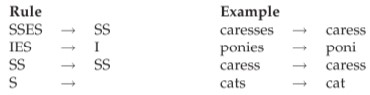
\includegraphics[scale = 1.8]{img/porter.jpg}
		\label{porter}
        \caption{Set of commands of the first phase}
\end{figure}

Many of the later rules use the concept of the \textit{measure} of a word, i.e. they check the number of syllables to see whether a word is long enough that is reasonable to regard the matching portion of a rule as a suffix rather than as part of the stem of a word. For example, the rule \textit{(m > 1) EMENT} would map \textit{replacement} to \textit{replac}, but not \textit{cement} to \textit{c} (since the prefix \textit{c} is not long enough).

In general, stemmers use language-specific rules, but they require less knowledge than a lemmatizer, which needs a complete vocabulary and morphological analysis to correctly lemmatize word. The \textbf{advantages} of performing stemming is that it helps increasing the \textbf{recall} of the IR system, i.e. the amount of its results, but on the other hand it could harm the precision, i.e. the quality of the results, of other IR system. In general, this operation helps on reducing the size of the vocabulary, and it was shown that is very useful for languages with much more morphology, such as Spanish, German and Finnish.
